\section{Kiểm tra time-series: stationarity, ACF/PACF và spectrum}

\subsection{Stationarity testing}

Theo yêu cầu môn học, báo cáo vẫn thực hiện ADF và KPSS trên aggregate series và các chuỗi đại diện. Tuy nhiên, với bài toán nhiều chuỗi bán lẻ, mục đích của stationarity test không phải để ép toàn bộ pipeline thành ARIMA cổ điển. Thay vào đó, ADF/KPSS giúp nhận diện mức độ trend/seasonality và củng cố quyết định dùng lag, rolling và seasonal baseline.


\begin{table}[H]
\centering
\caption{Kết quả ADF/KPSS}
\label{tab:long-stationarity}
\resizebox{\linewidth}{!}{%
\begin{tabular}{llllll}
\toprule
Series & Transformation & ADF p-value & KPSS p-value & Conclusion & N \\
\midrule
aggregate\_hourly\_sales & original & 0.0000 & 0.0100 & mixed evidence & 2328 \\
aggregate\_hourly\_sales & log1p & 0.0000 & 0.0100 & mixed evidence & 2328 \\
aggregate\_hourly\_sales & first\_difference & 0.0000 & 0.1000 & stationary & 2327 \\
aggregate\_hourly\_sales & seasonal\_difference\_lag\_24 & 0.0000 & 0.1000 & stationary & 2304 \\
high\_volume\_series & original & 0.3070 & 0.0100 & non-stationary & 2328 \\
high\_volume\_series & log1p & 0.4265 & 0.0100 & non-stationary & 2328 \\
high\_volume\_series & first\_difference & 0.0000 & 0.1000 & stationary & 2327 \\
high\_volume\_series & seasonal\_difference\_lag\_24 & 0.0000 & 0.1000 & stationary & 2304 \\
intermittent\_series & original & 0.0000 & 0.1000 & stationary & 2328 \\
intermittent\_series & log1p & 0.0000 & 0.1000 & stationary & 2328 \\
intermittent\_series & first\_difference & 0.0000 & 0.1000 & stationary & 2327 \\
intermittent\_series & seasonal\_difference\_lag\_24 & 0.0000 & 0.1000 & stationary & 2304 \\
stockout\_heavy\_series & original & 0.0058 & 0.0100 & mixed evidence & 2328 \\
stockout\_heavy\_series & log1p & 0.0031 & 0.0100 & mixed evidence & 2328 \\
stockout\_heavy\_series & first\_difference & 0.0000 & 0.1000 & stationary & 2327 \\
stockout\_heavy\_series & seasonal\_difference\_lag\_24 & 0.0000 & 0.1000 & stationary & 2304 \\
\bottomrule
\end{tabular}
}
\end{table}


\subsection{ACF/PACF}

ACF/PACF cho thấy autocorrelation và seasonal dependence ở các lag ngắn và lag theo ngày/tuần. Với dữ liệu hourly, lag 24 và 168 có ý nghĩa tự nhiên. Trong pipeline cuối, recovery được làm ở cấp hourly, còn forecasting được aggregate lên daily và dùng lag 7/14/28 ngày.


\begin{figure}[H]
    \centering
    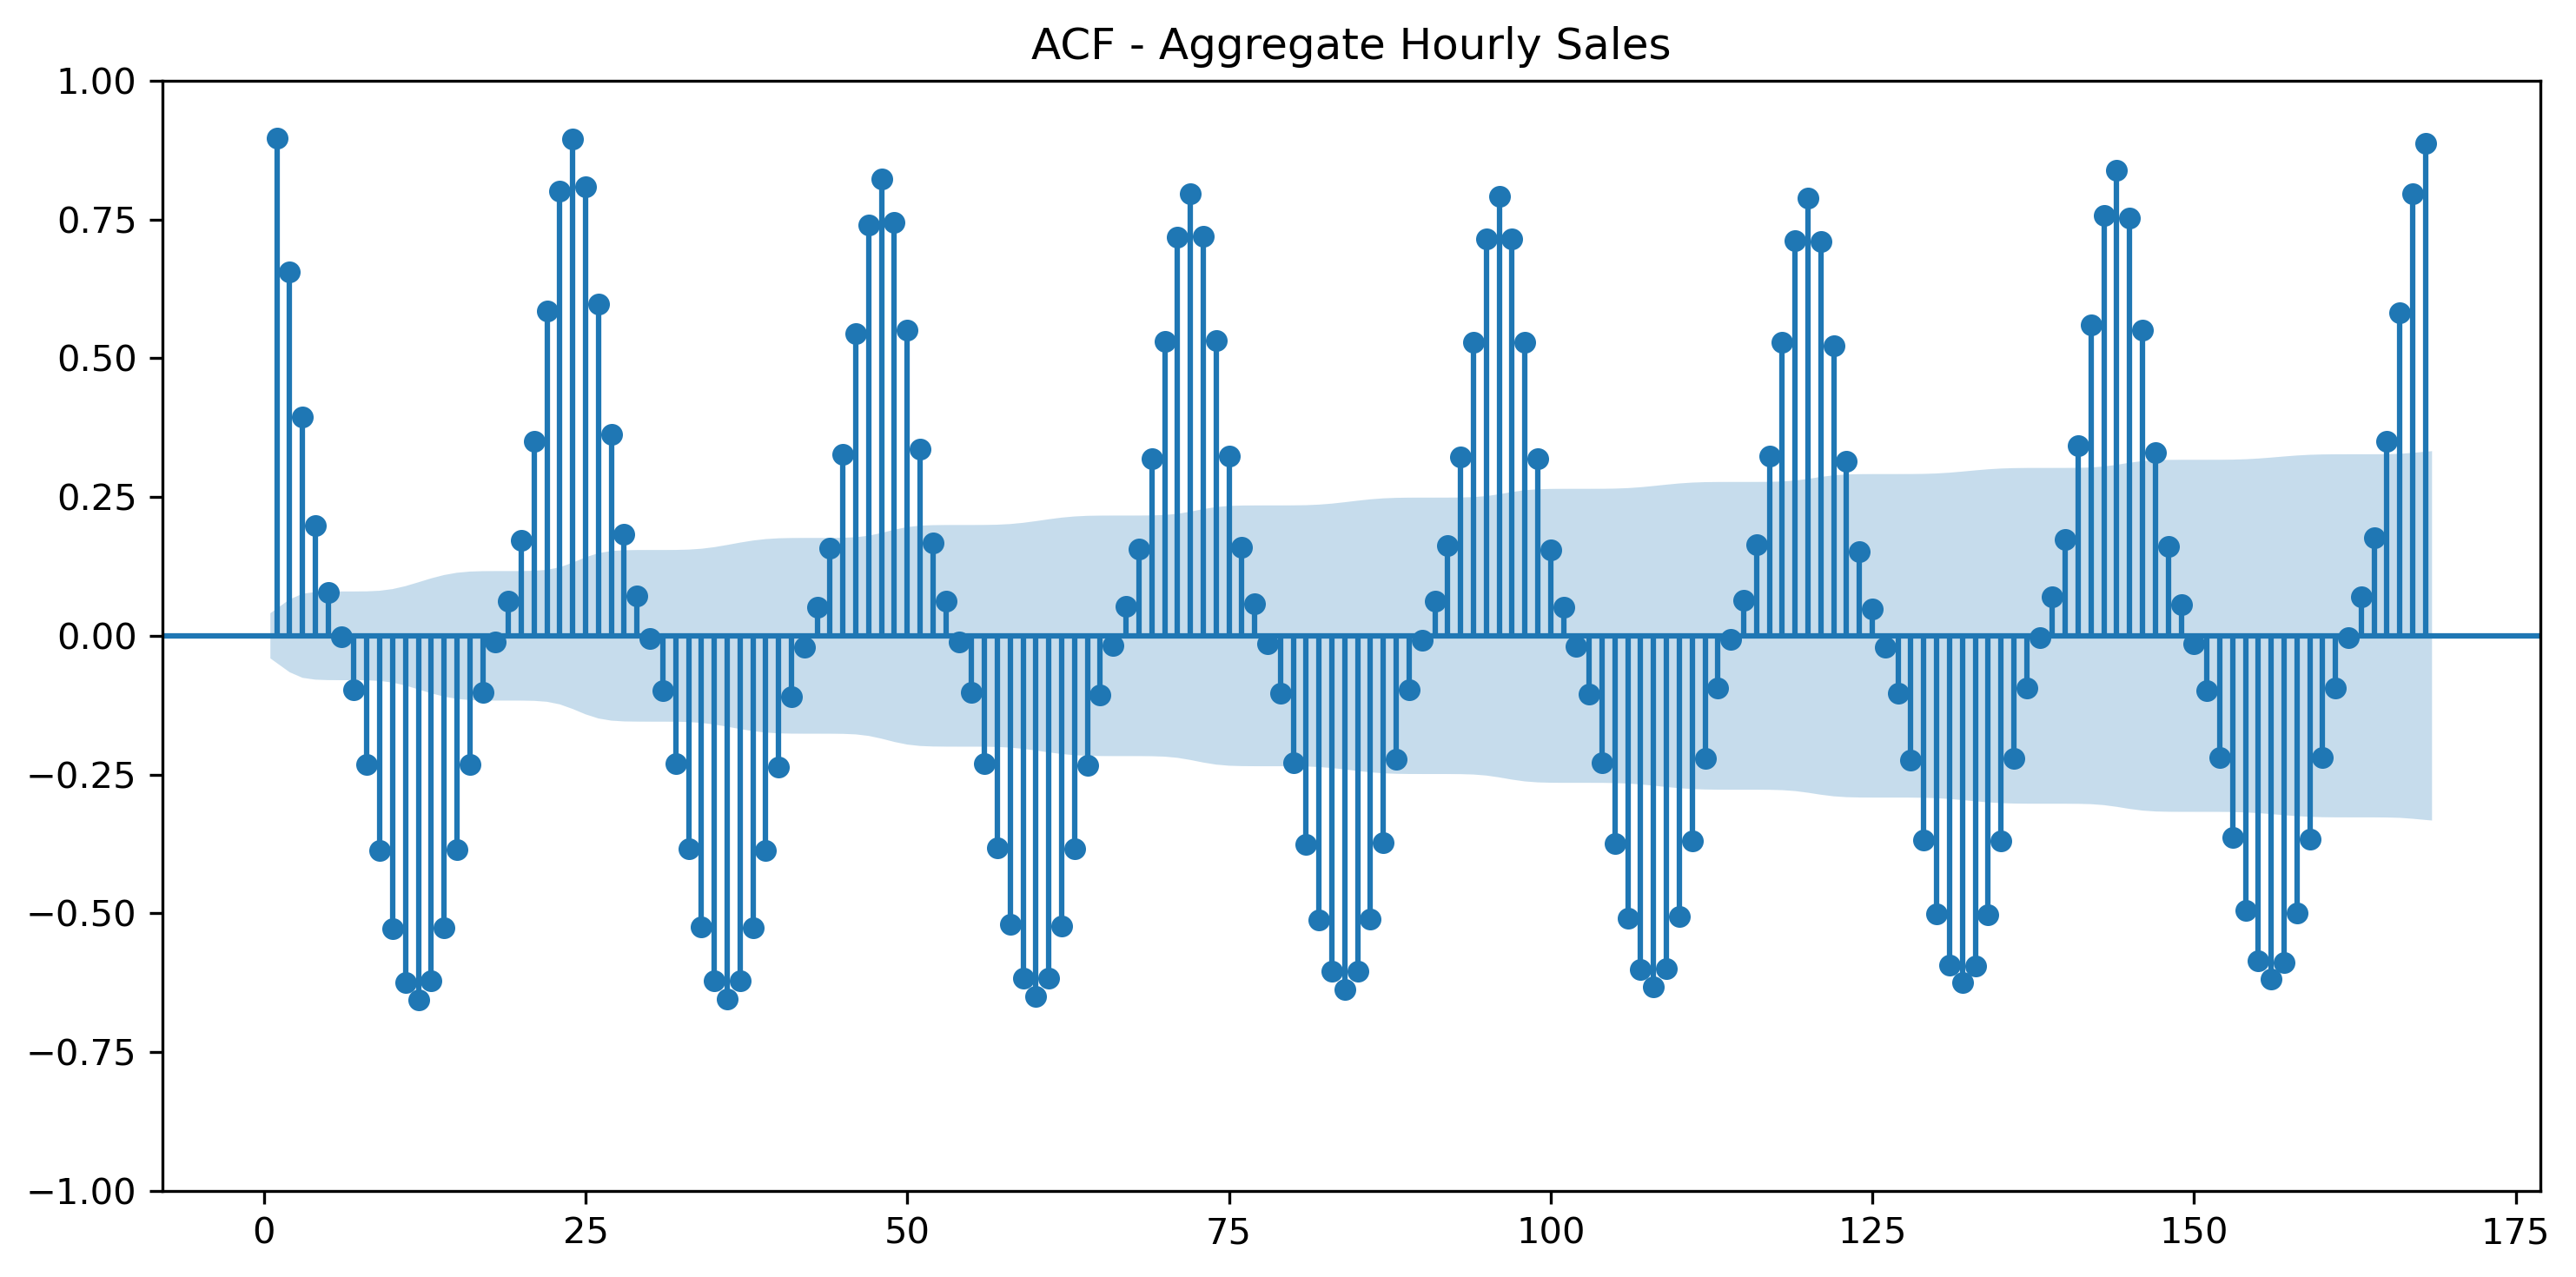
\includegraphics[width=0.84\linewidth]{figures/acf_aggregate_sales.png}
    \caption{ACF của aggregate hourly sales.}
    \label{fig:long-acf-agg}
\end{figure}



\begin{figure}[H]
    \centering
    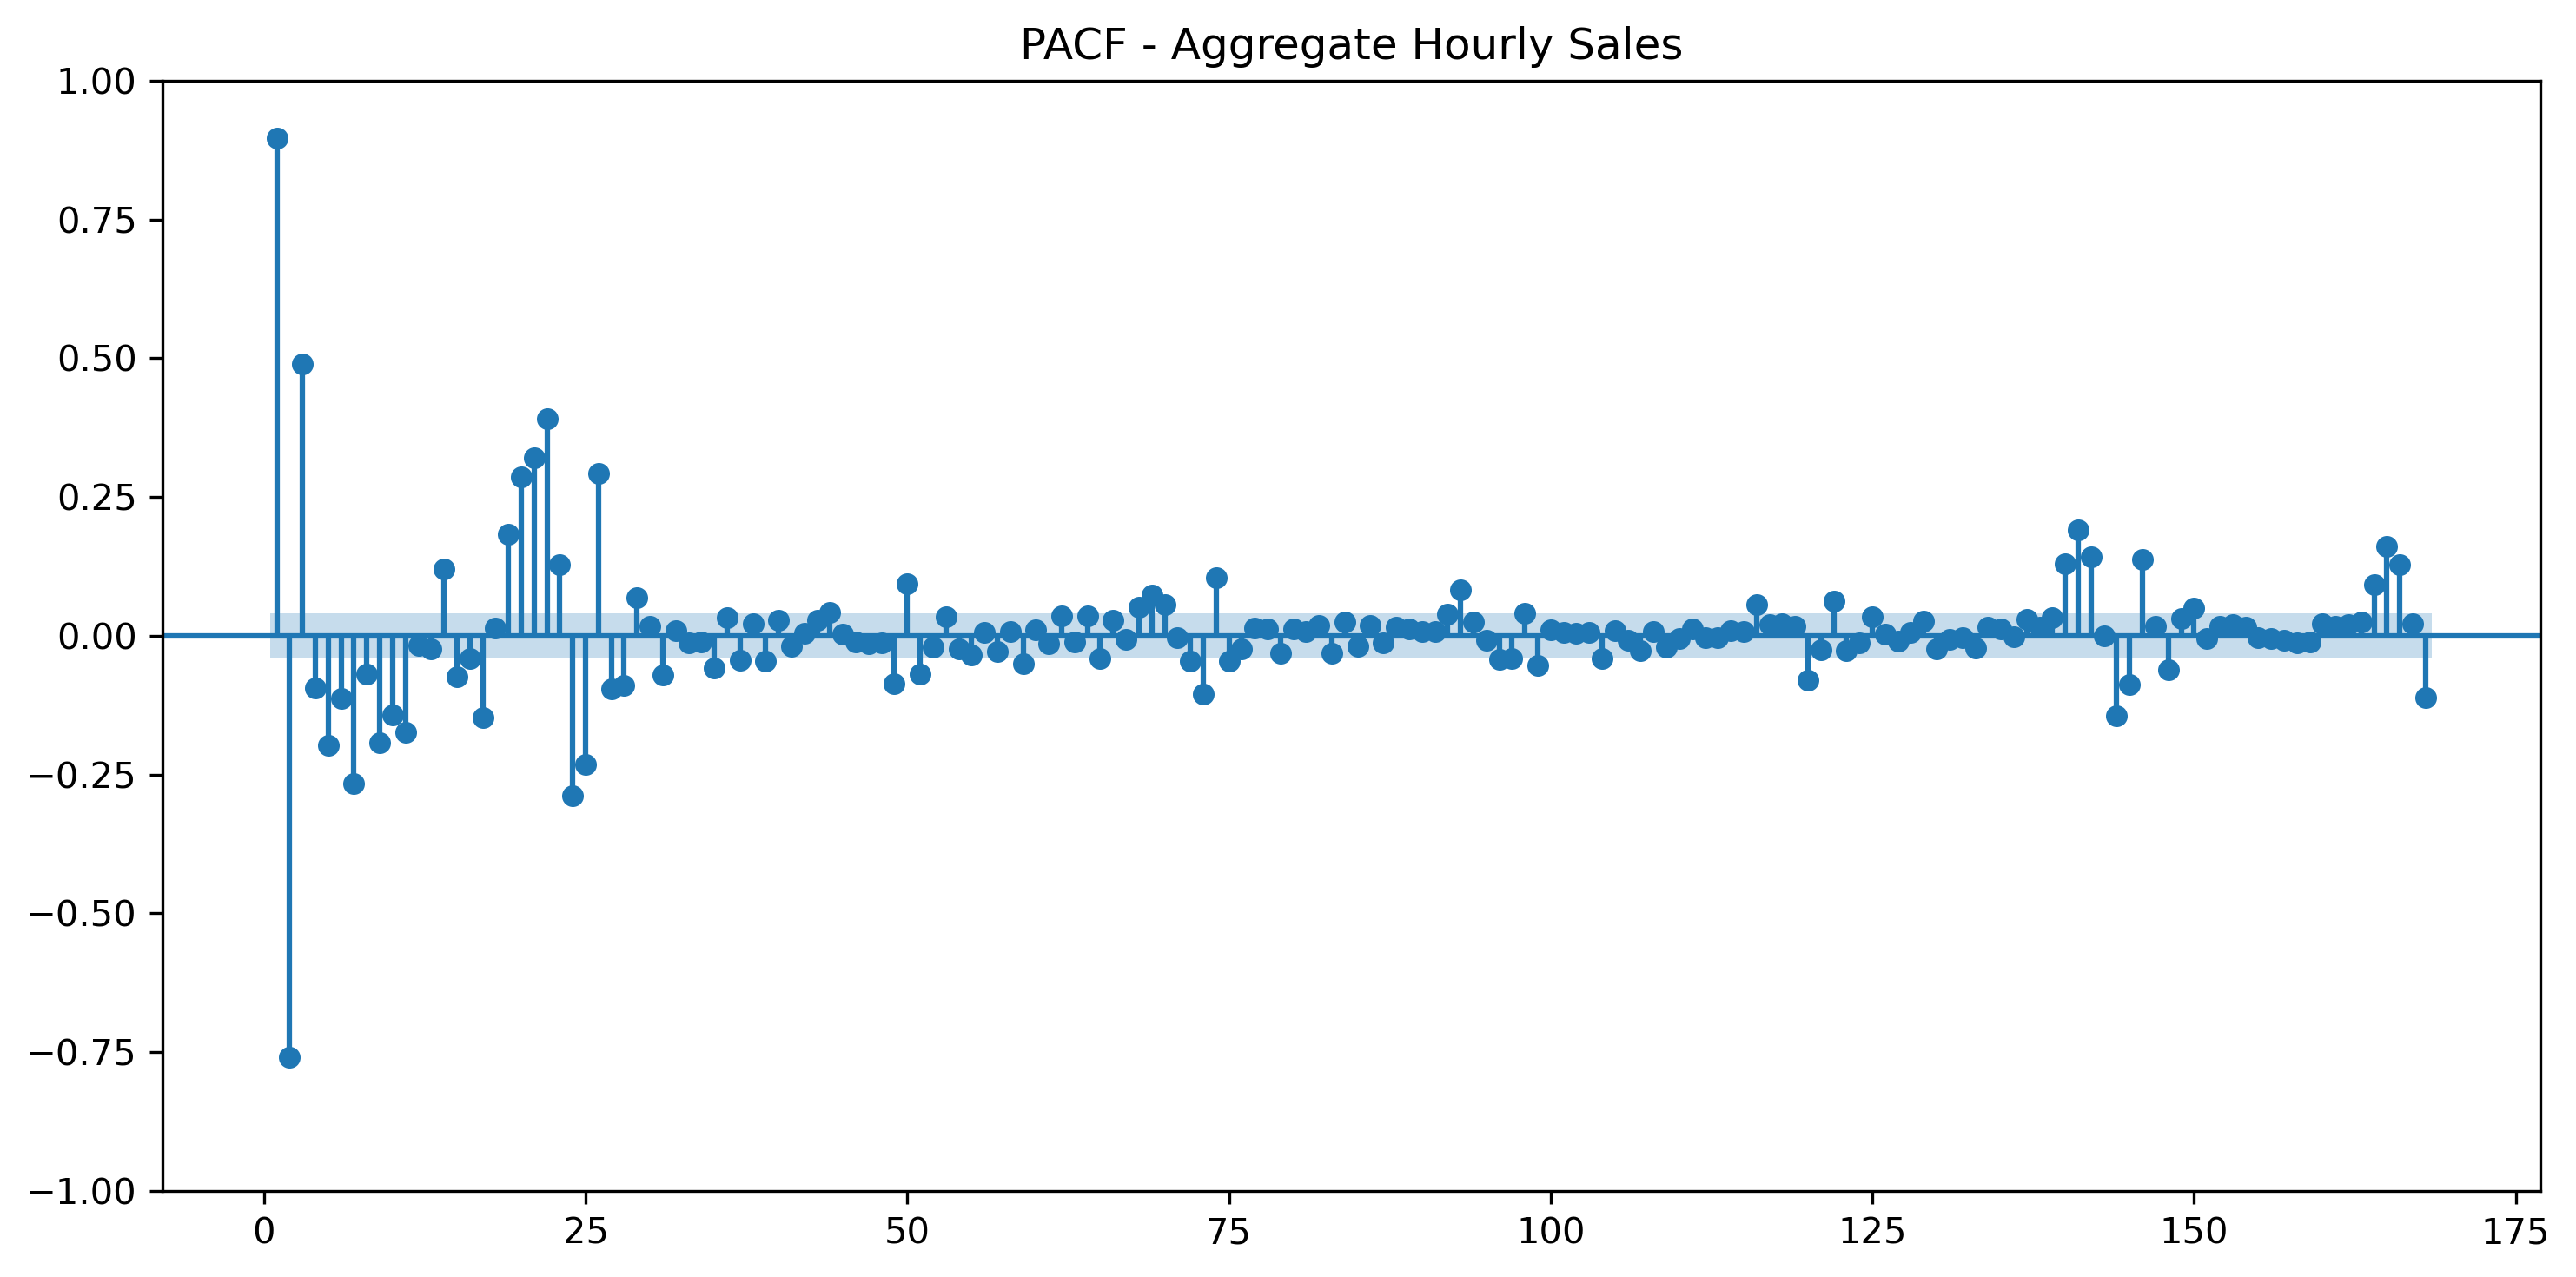
\includegraphics[width=0.84\linewidth]{figures/pacf_aggregate_sales.png}
    \caption{PACF của aggregate hourly sales.}
    \label{fig:long-pacf-agg}
\end{figure}



\begin{figure}[H]
    \centering
    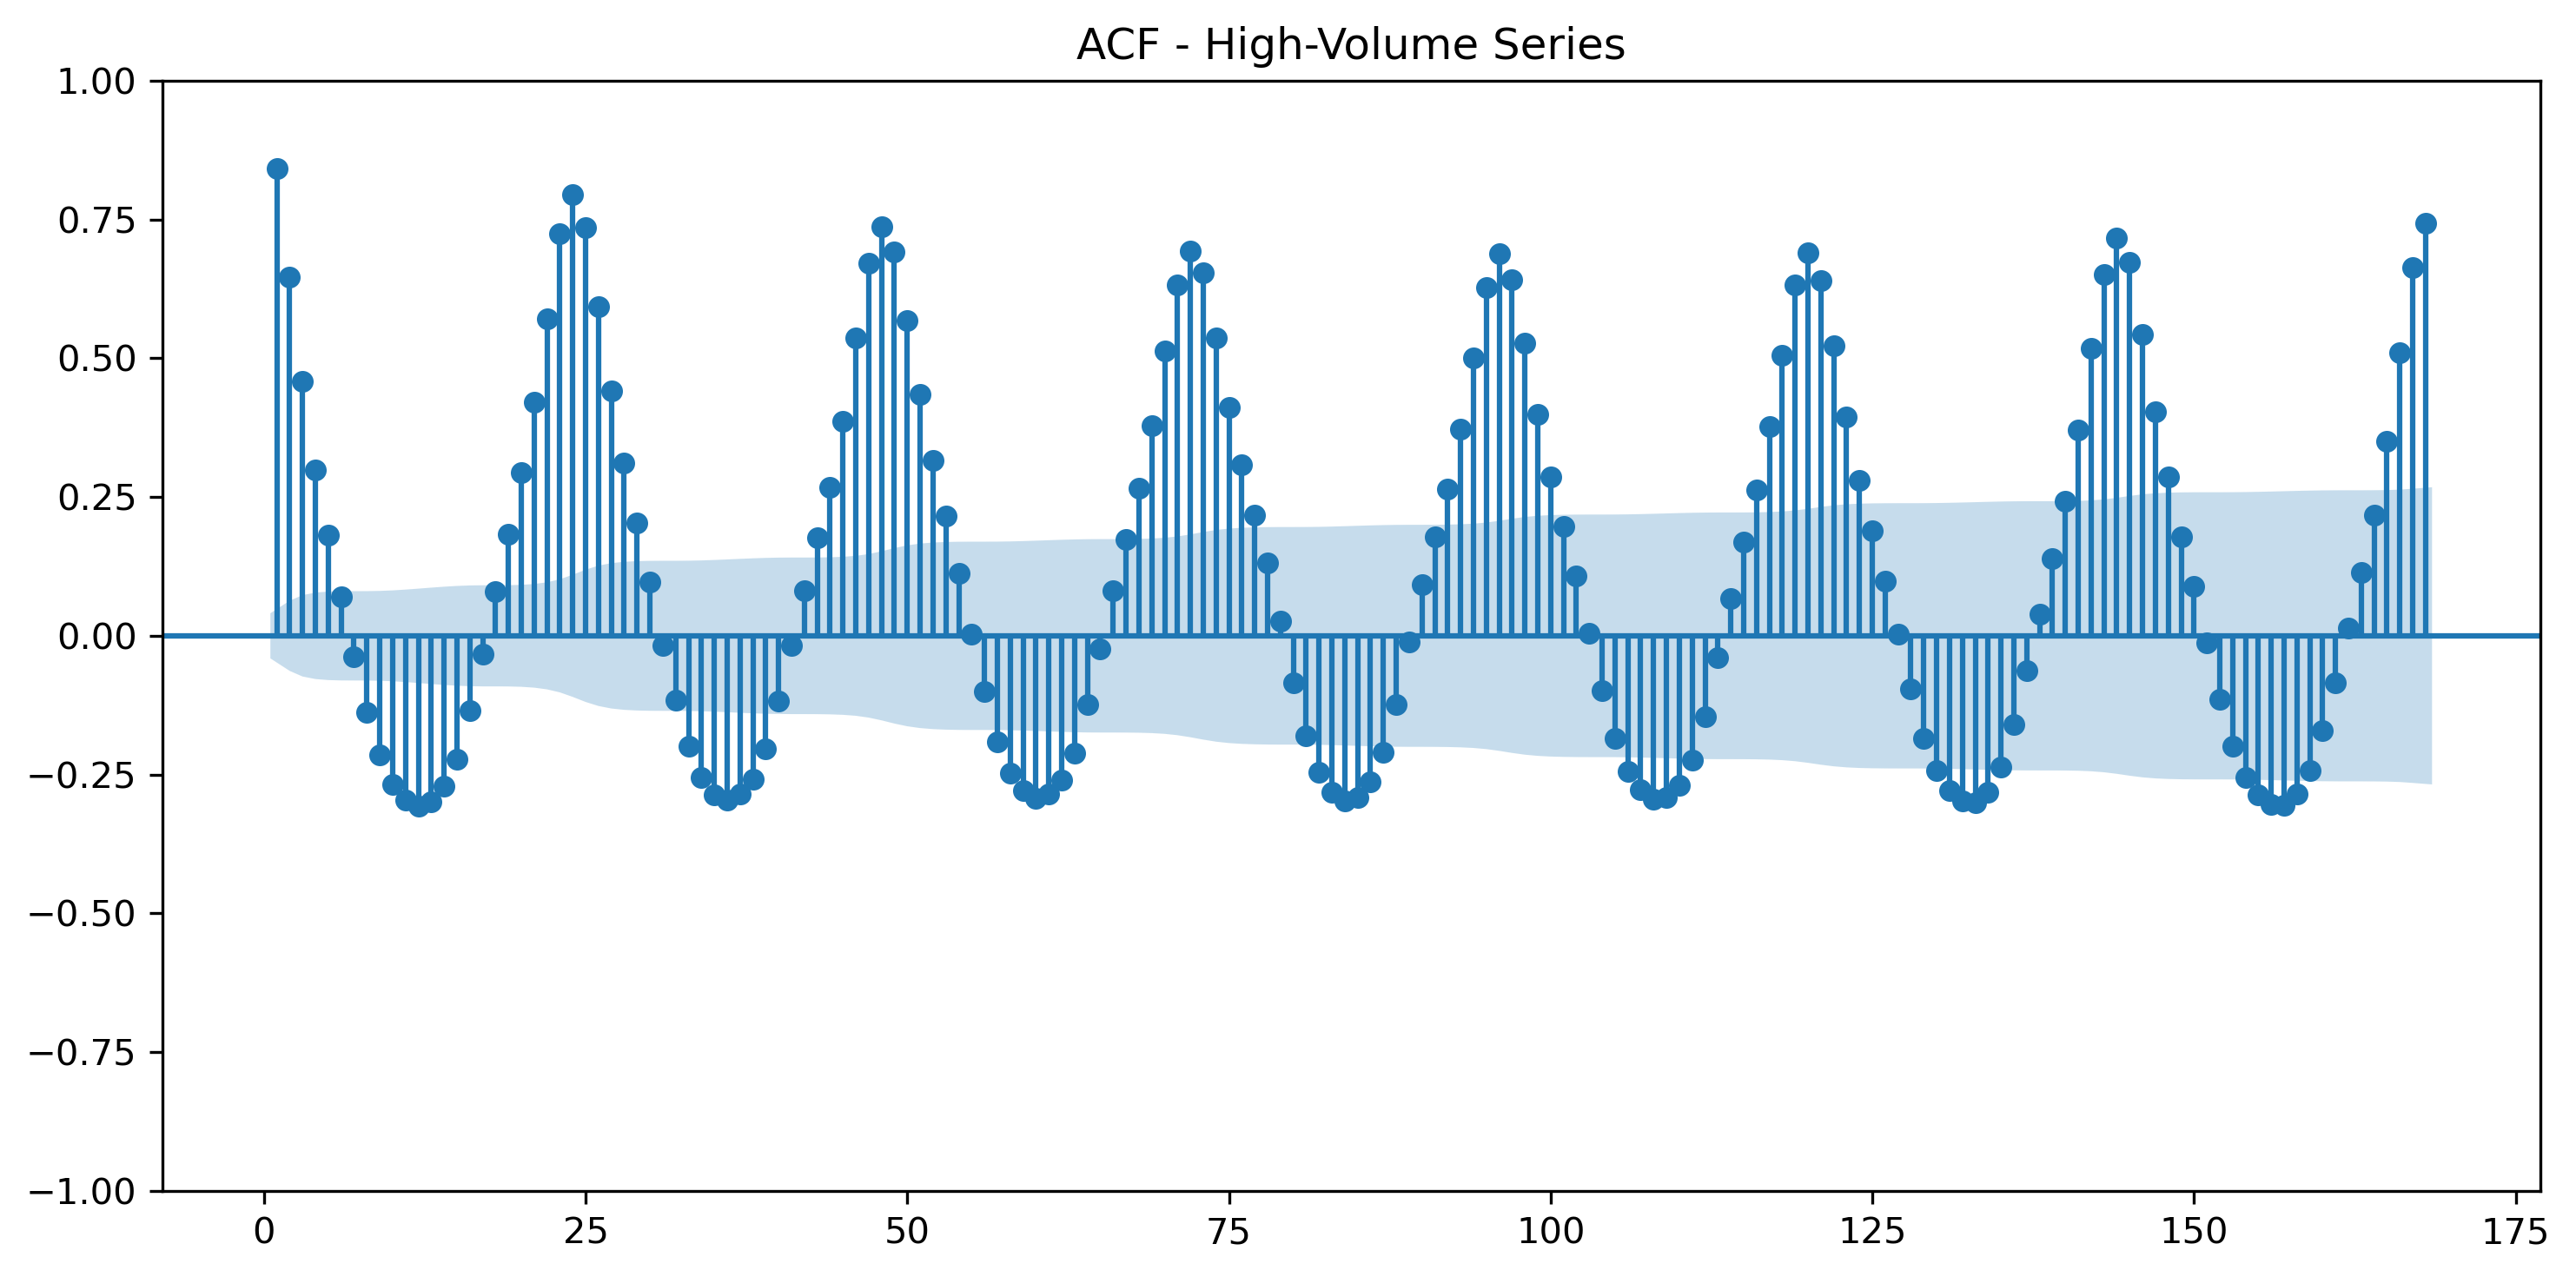
\includegraphics[width=0.84\linewidth]{figures/acf_high_volume_series.png}
    \caption{ACF của chuỗi high-volume.}
    \label{fig:long-acf-high}
\end{figure}



\begin{figure}[H]
    \centering
    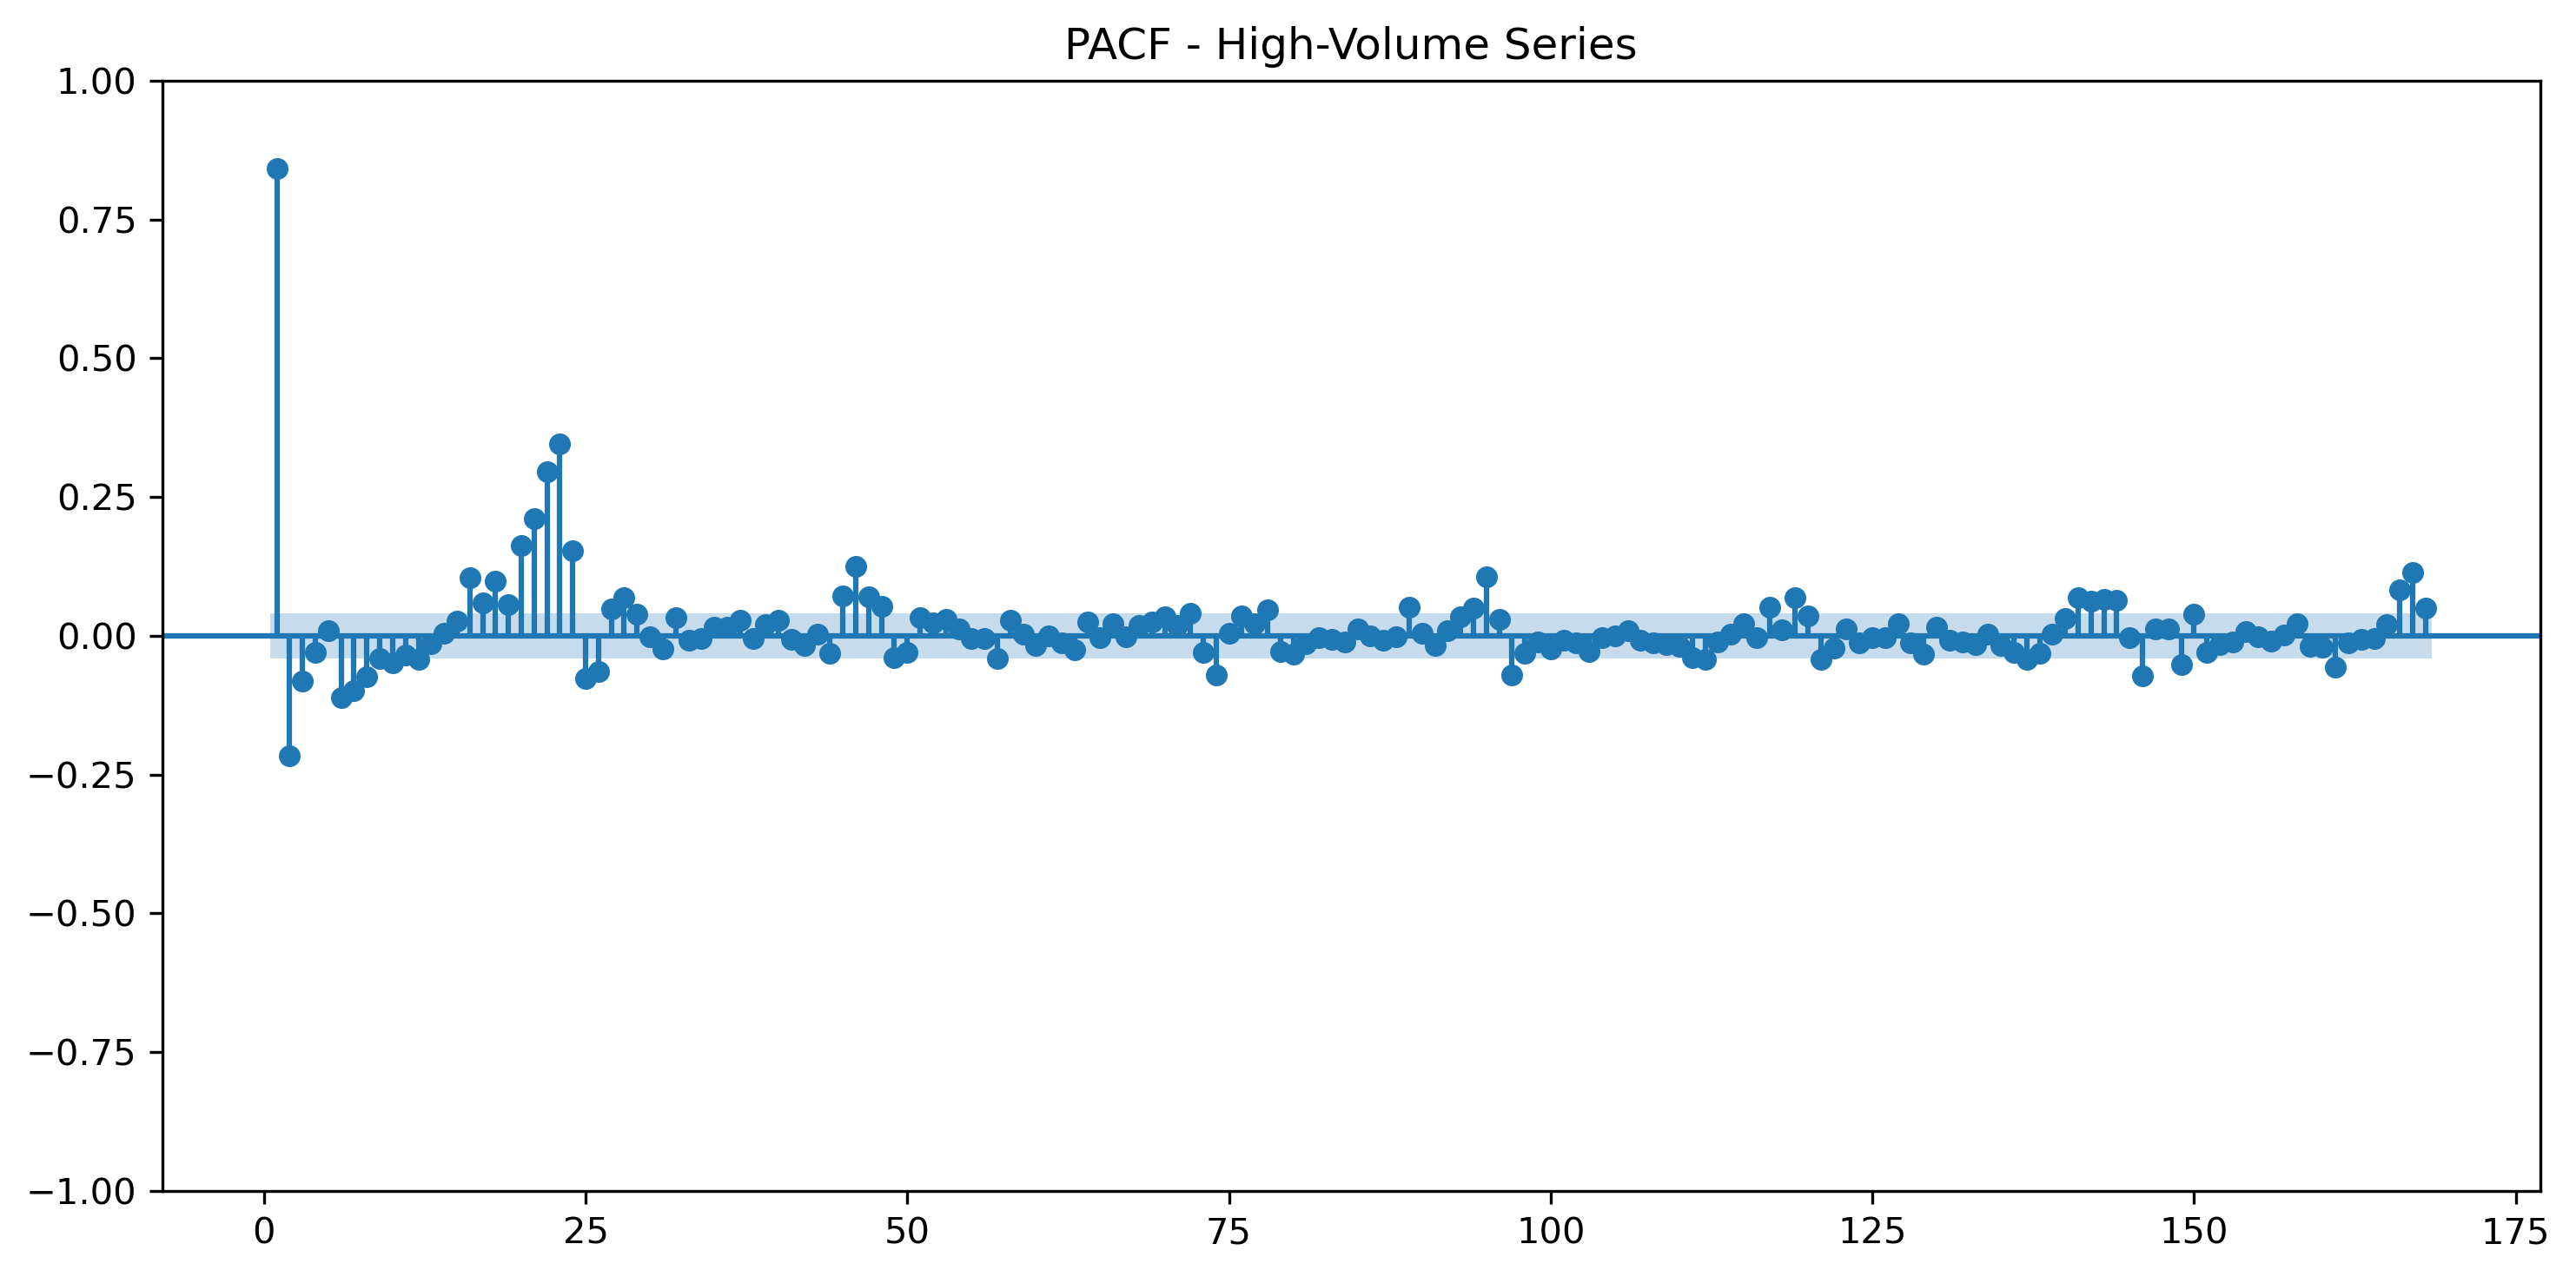
\includegraphics[width=0.84\linewidth]{figures/pacf_high_volume_series.png}
    \caption{PACF của chuỗi high-volume.}
    \label{fig:long-pacf-high}
\end{figure}


\subsection{Spectrum analysis}

Periodogram được dùng như một cách kiểm tra độc lập trong miền tần số. Hourly aggregate sales có peak mạnh quanh 24 giờ, còn daily recovered demand có peak gần 7 ngày. Điều này giải thích vì sao seasonal naive 7 ngày không phải baseline yếu mà là benchmark rất khó đánh bại.


\begin{figure}[H]
    \centering
    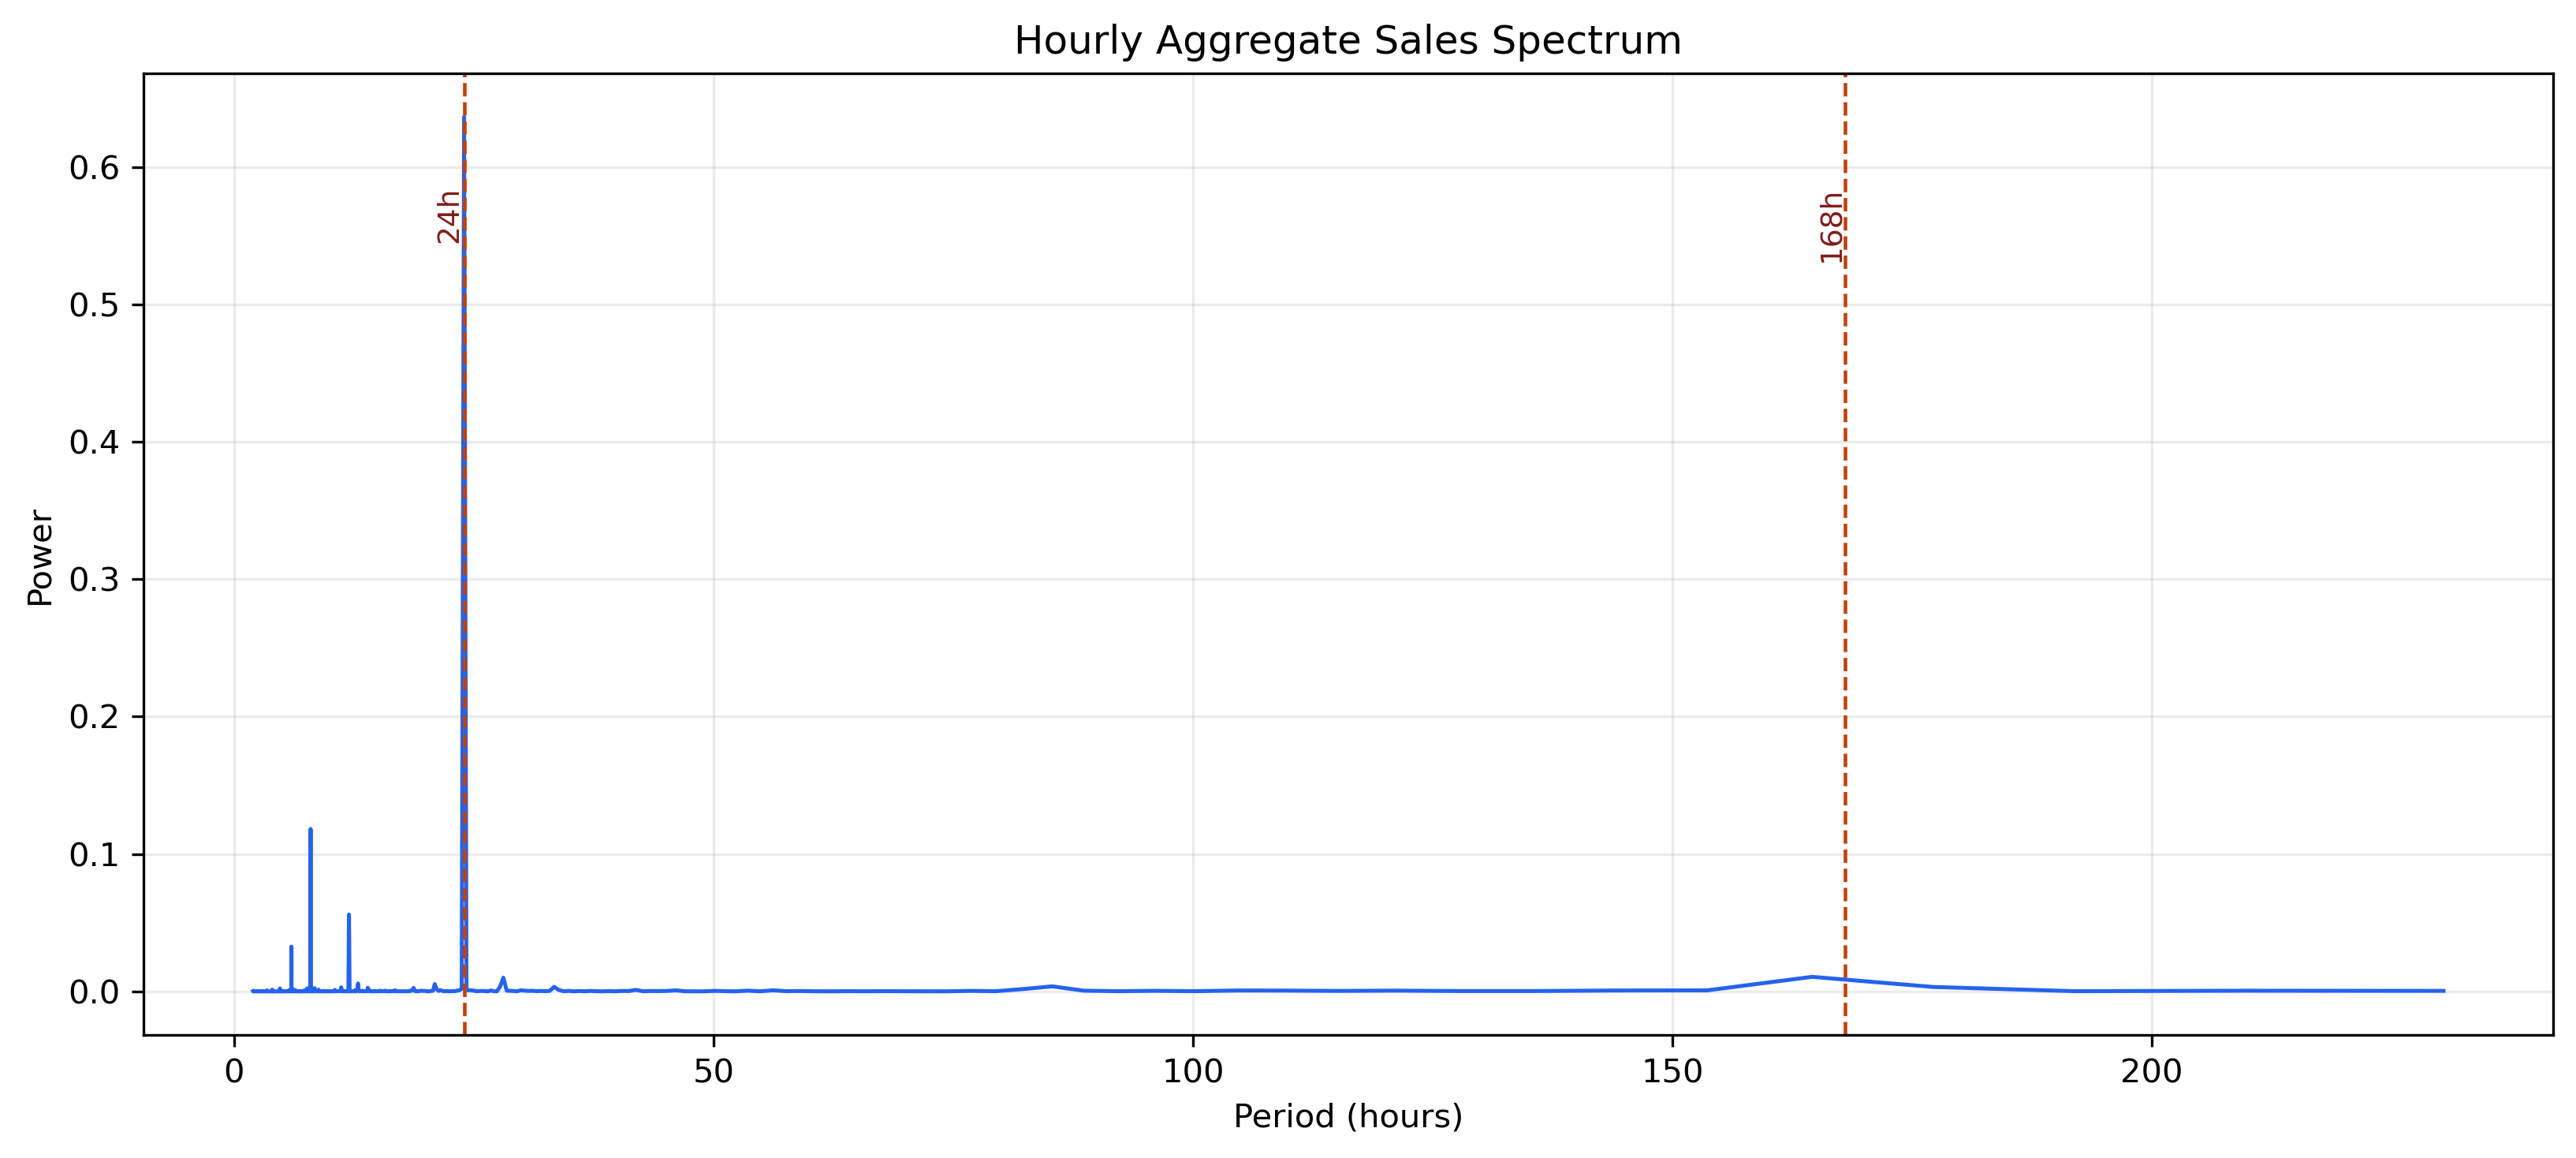
\includegraphics[width=0.86\linewidth]{figures/spectrum_hourly_aggregate_sales.png}
    \caption{Spectrum của hourly aggregate observed sales.}
    \label{fig:long-spectrum-hourly}
\end{figure}



\begin{table}[H]
\centering
\caption{Các peak spectrum hourly}
\label{tab:long-spectrum-hourly}
\resizebox{\linewidth}{!}{%
\begin{tabular}{lllll}
\toprule
Rank & Period & Frequency & Power & Period unit \\
\midrule
1 & 24.0000 & 0.0417 & 0.6365 & hours \\
2 & 8.0000 & 0.1250 & 0.1182 & hours \\
3 & 12.0000 & 0.0833 & 0.0559 & hours \\
4 & 6.0000 & 0.1667 & 0.0325 & hours \\
5 & 164.5714 & 0.0061 & 0.0106 & hours \\
6 & 28.0976 & 0.0356 & 0.0099 & hours \\
7 & 12.9438 & 0.0773 & 0.0058 & hours \\
8 & 20.9455 & 0.0477 & 0.0053 & hours \\
\bottomrule
\end{tabular}
}
\end{table}



\begin{figure}[H]
    \centering
    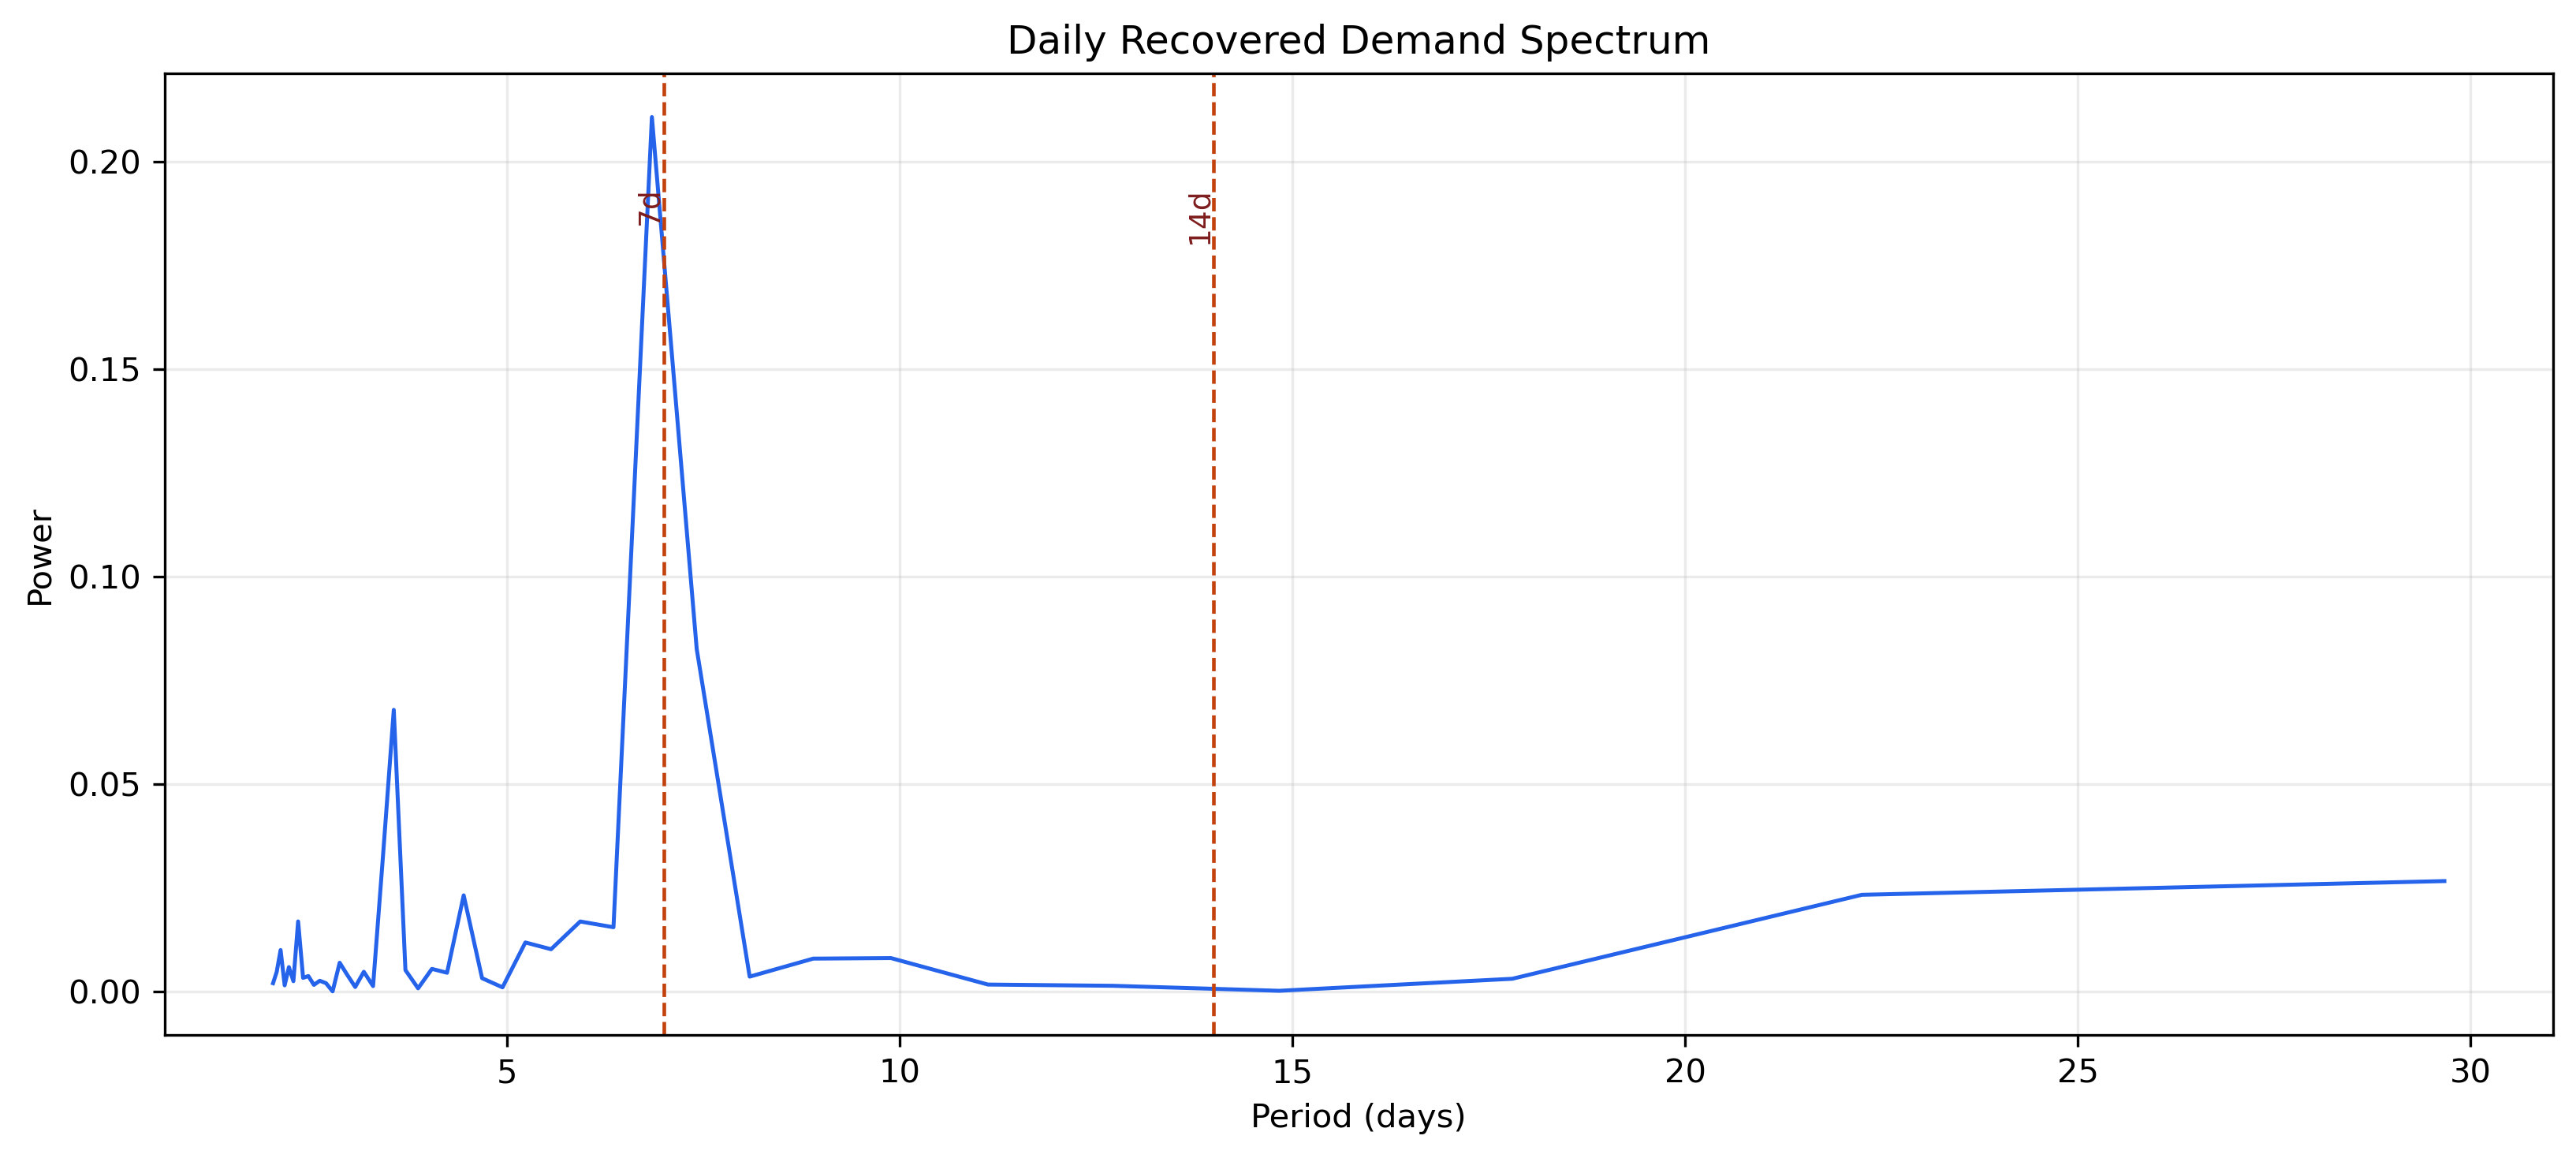
\includegraphics[width=0.86\linewidth]{figures/spectrum_daily_recovered_demand.png}
    \caption{Spectrum của daily recovered demand.}
    \label{fig:long-spectrum-daily}
\end{figure}



\begin{table}[H]
\centering
\caption{Các peak spectrum daily}
\label{tab:long-spectrum-daily}
\resizebox{\linewidth}{!}{%
\begin{tabular}{lllll}
\toprule
Rank & Period & Frequency & Power & Period unit \\
\midrule
1 & 6.8462 & 0.1461 & 0.2108 & days \\
2 & 3.5600 & 0.2809 & 0.0679 & days \\
3 & 4.4500 & 0.2247 & 0.0232 & days \\
4 & 2.3421 & 0.4270 & 0.0169 & days \\
5 & 5.9333 & 0.1685 & 0.0169 & days \\
6 & 5.2353 & 0.1910 & 0.0118 & days \\
7 & 2.1190 & 0.4719 & 0.0100 & days \\
8 & 9.8889 & 0.1011 & 0.0081 & days \\
\bottomrule
\end{tabular}
}
\end{table}
